


Figures \ref{fig:mosaic_dry} and \ref{fig:mosaic_wet} illustrate the temporal development of forest cover in the two study regions. In the dry forest (fig. \ref{fig:mosaic_dry}), the majority of the forest landscape is covered by late successional forest ($>30\ years$), while most early successional forest ($\le30\ years$) only began regrowing in the late 2010s. In contrast, the wet tropical forest (fig. \ref{fig:mosaic_wet}) contains a larger proportion of non-forest cover, with late successional forest primarily concentrated in the northern part of the \ac{ROI}. Early successional forest in this region also shows regrowth beginning mainly from the late 2010s. A more detailed overview of forest distribution across different buffer radii within the \ac{ROI} is provided in appendix~\ref{app:spatial_distri} and illustrated in figures \ref{fig:radius_dry} and \ref{fig:radius_wet}.

\begin{figure}[htb]
\centering
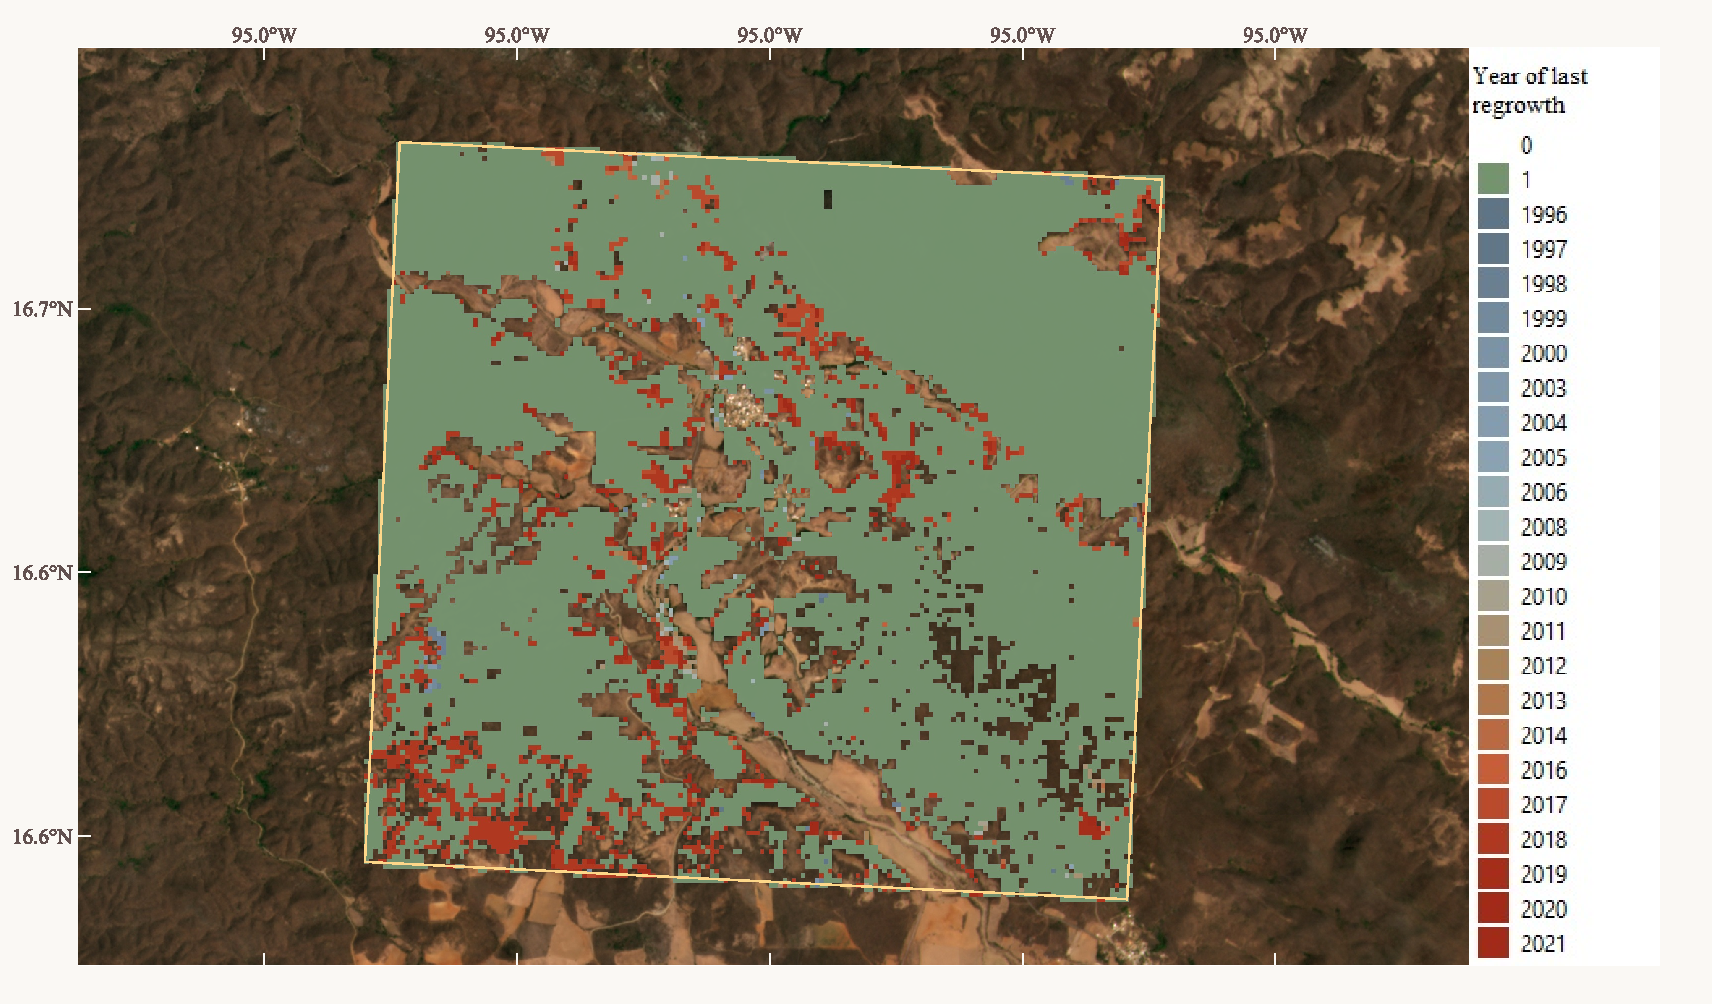
\includegraphics[width=\linewidth, keepaspectratio]{Report/figures/08_forestmosaic_dry.pdf}
\caption{\textit{Last regrowth in the surrounding forest landscape of the dry tropical forest. The color of each pixel indicates the year of last regrowth—the first year of a secondary tropical forest (within the temporal limits of this study). A value of 0 (transparent) represents non-forest areas, and a value of 1 (green) represents old-growth forest—forests older than 30 years (the temporal boundary of our study). This map was derived from the \ac{AVOCADO} algorithm developed by \citet{decuyperContinuousMonitoringForest2022}.}}
\label{fig:mosaic_dry}
\end{figure}

\begin{figure}[htb]
\centering
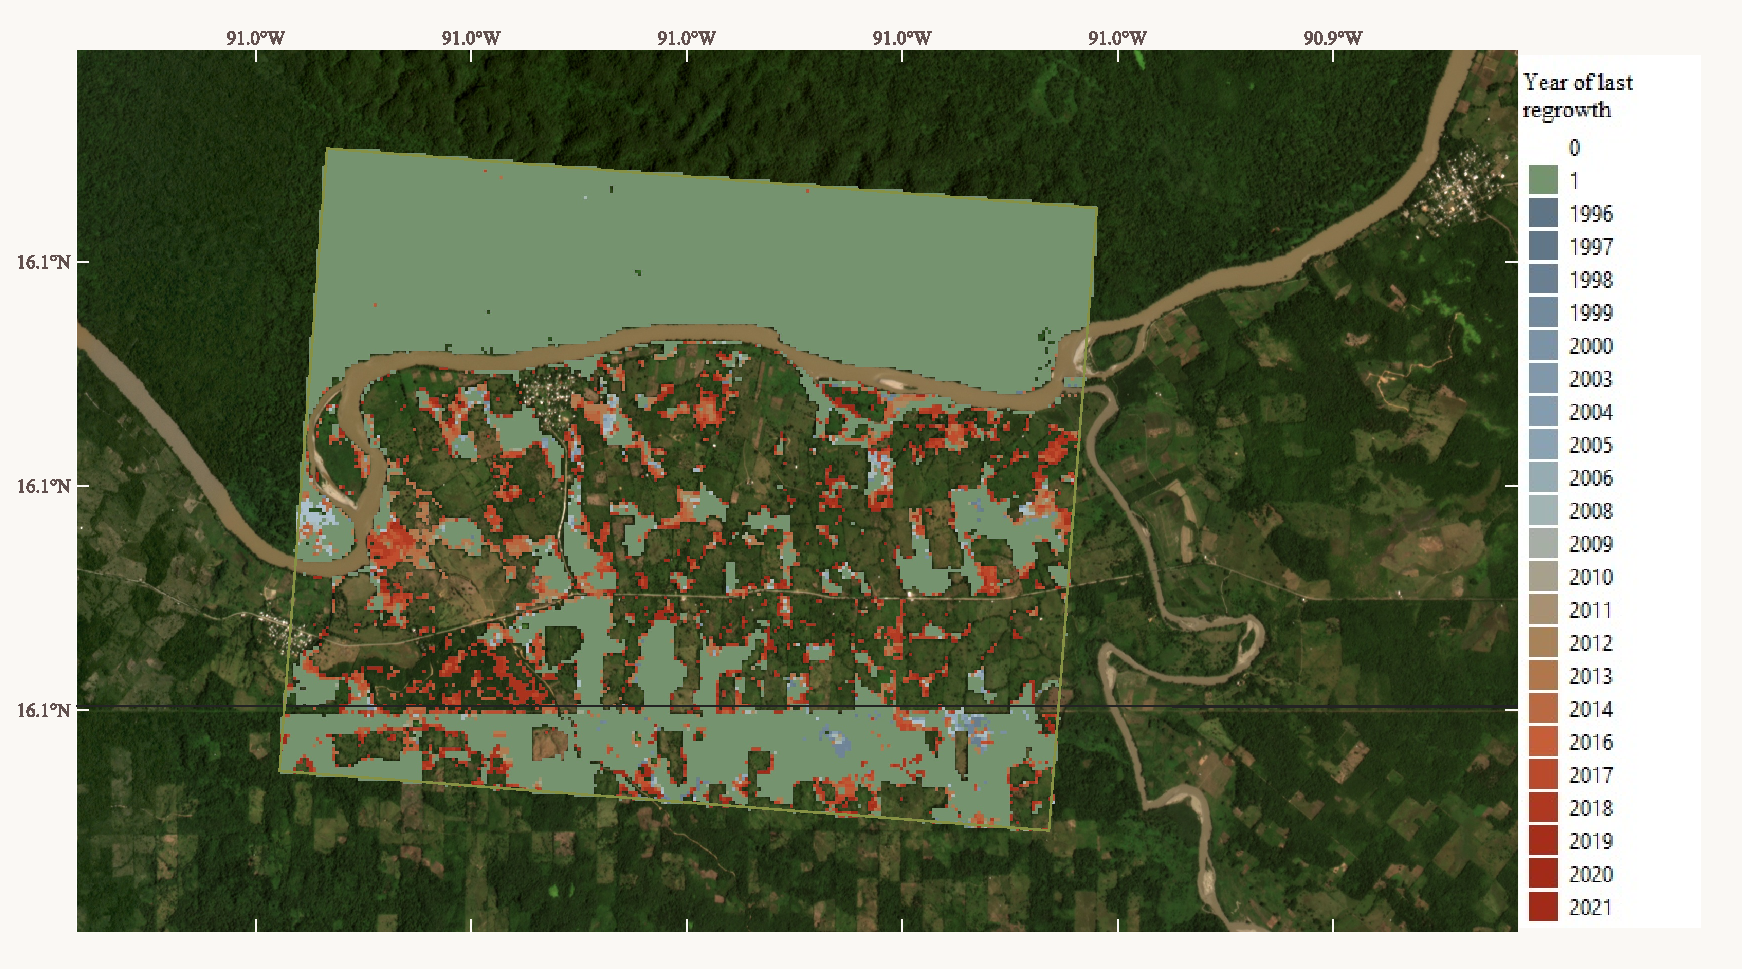
\includegraphics[width=\linewidth, keepaspectratio]{Report/figures/09_forestmosaic_wet.pdf}
\caption{\textit{Last regrowth in the surrounding forest landscape of the wet tropical forest. The color of a pixel indicates the last year of regrowth - the first year of a secondary tropical forest (within the temporal limits of this study). A value of 0 (transparent) represents non-forest areas, and a value of 1 (green) represents old-growth forest—forests older than 30 years (the temporal boundary of our study). This map was derived from the \ac{AVOCADO} algorithm developed by \citet{decuyperContinuousMonitoringForest2022}.}}
\label{fig:mosaic_wet}
\end{figure}

\subsection{Spearman's correlation}
Spearman's correlation analysis was performed to statistically analyse the relationships among numeric variables in dry and wet tropical forest (fig. \ref{fig:cor}). 
In dry tropical forest, a moderately significant positive correlation was observed between generalist guild and early successional forest ($\rho = 0.52, p < 0.05$) and marginally significant negative relationships were observed between shade-tolerant guild and early successional forest ($\rho = -0.41, p < 0.1$), generalist and forest cover ($\rho = -0.38, p < 0.1$), and richness and forest connectivity ($\rho = -0.39, p < 0.1$).
In wet tropical forests, a moderately significant positive correlation was observed between richness and forest cover ($\rho = 0.5, p < 0.05$) and marginally significant negative relationship was observed between richness and early successional forest ($\rho = -0.39, p < 0.1$).

\begin{figure}[htb]
\centering
\setlength{\fboxrule}{12pt}  % thickness of the frame
\setlength{\fboxsep}{0pt}   % no padding between frame and image
\fcolorbox{framecol}{white}{%
  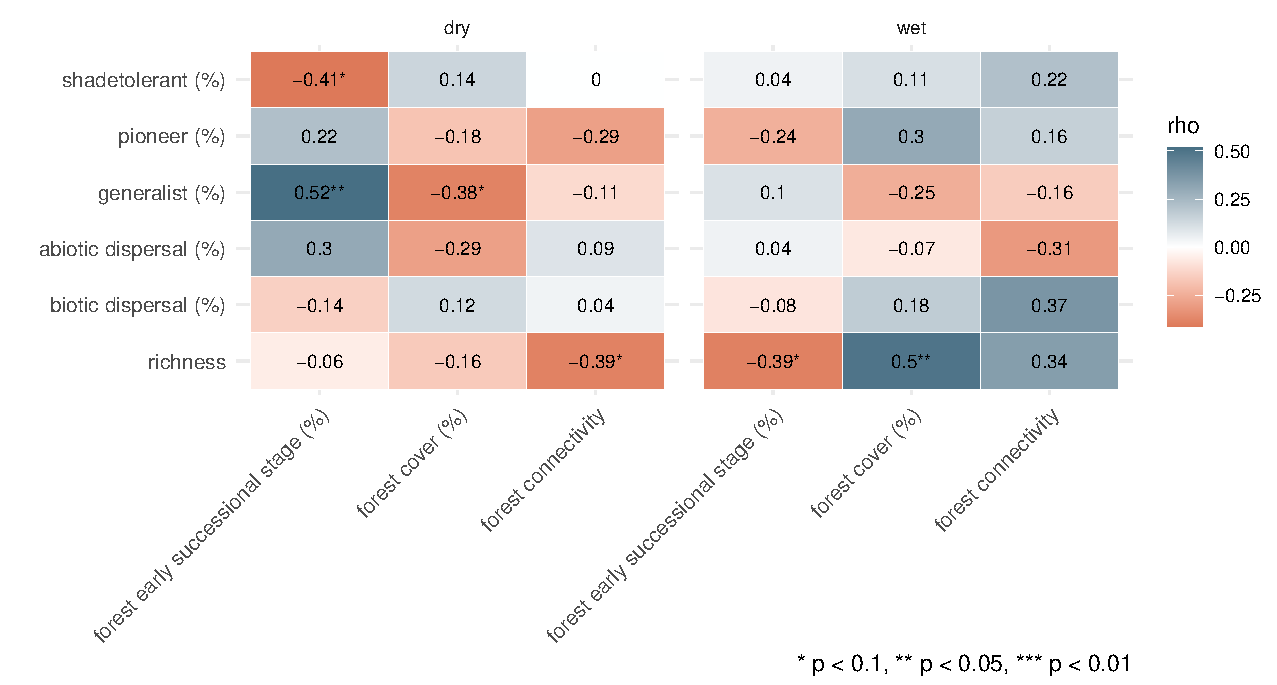
\includegraphics[width=\linewidth, keepaspectratio]{Report/figures/10_correlation.pdf}%
}
\caption{\textit{Spearman's rank correlation matrix. Number inside each cells represents correlation coefficient (Spearman's rho). Additionally, asterix is an indicative of a significance of the relationship (*p $<$ 0.1, **p $<$ 0.05, ***p $<$ 0.01).}}
\label{fig:cor}
\end{figure}

\subsection{Linear model results}


\textbf{Seed richness:}
The linear regression models with seed richness as the dependent variable showed a significant overall effect ($F(3, 36) = 11.44$–$12.45$, $p < 0.01$), explaining 44.5\% of the variance in model 1 (forest cover, connectivity, and forest type) and 46.8\% in models 2 and 3 (successional stage, connectivity, and forest type). 
In all models, \textbf{forest type} was the main significant predictor ($\beta = 9.624$–$11.044$, $p < 0.01$), with wet forests showing significantly higher seed richness than dry forests (tab. \ref{tab:sum_mods}; fig \ref{fig:stats}). 
In models 2 and 3, \textbf{successional stage} also had a marginal effect ($p < 0.1$): early successional stage showed a negative effect on seed richness ($\beta = -2.652$), while late successional stage had a positive effect ($\beta = 2.652$) (tab. \ref{tab:sum_mods}; fig \ref{fig:stats}). 
See appendix \ref{app:mod_res} (tab. \ref{tab:richness}; fig. \ref{fig:mod_richness}) for detailed model results.

\textbf{Seed dispersal mode:}
The linear regression models with percentage of biotically dispersed seeds as the dependent variable showed a significant overall effect $(F(3, 36) = 21.632 - 21.852, p < 0.01)$, explaining 61.6\% of variance in model 1 (forest cover, forest connectivity and forest type)  and 61.3\% of variance in model 2 and 3 (forest successional stage, forest connectivity and forest type). In all models, \textbf{forest type} was the only significant predictor $(\beta = 0.530 - 0.526, p < 0.01)$, indicating a significantly higher biotic seed dispersal in the wet forest type compared to the dry forest type (tab. \ref{tab:sum_mods}; fig \ref{fig:stats}). See appendix \ref{app:mod_res} (tab. \ref{tab:biotic}; fig. \ref{fig:mod_biotic}) for detailed model results.

The linear regression models with percentage of abiotically dispersed seeds as the dependent variable showed a significant overall effect $(F(3, 36) = 7.435 - 8.282, p<0.01)$, explaining 35.9\% of variance in model 1 (forest cover, forest connectivity and forest type) and 33.1\% of variance in model 2 and 3 (forest successional stage, forest connectivity and forest type). In all models, \textbf{forest type} is the main significant predictor $(\beta = -0.473 - (-0.429), p < 0.01)$, indicating a significantly lower abiotic dispersal in the wet forest compared to the dry forest type (tab. \ref{tab:abiotic}; fig. \ref{fig:stats}). See appendix \ref{app:mod_res} (tab. \ref{tab:abiotic}; fig. \ref{fig:mod_abiotic}) for detailed model results. 

\textbf{Seed guild:}
The linear regression models with percentage of seeds belonging to generalist species as the dependent variable showed a significant overall effect $(F(3, 36 = 3.599, p<0.05)$, explaining 16.7\% of variance in model 1 (forest cover, forest connectivity, forest type). In this model a higher \textbf{forest cover} was related to a lower percentage of generalist species dispersed $(\beta = -0.074, p < 0.05)$ (tab. \ref{tab:sum_mods}, fig. \ref{fig:stats}). The model 2 and 3 were not statistically significant. See appendix \ref{app:mod_res} (tab. \ref{tab:generalist}; fig. \ref{fig:mod_generalist}) for detailed model results. 

The linear regression models with percentage of seeds belonging to pioneer and shade-tolerant species as the dependent variables did not show any significant relationships. See appendix \ref{app:mod_res} (tab. \ref{tab:pioneer}, \ref{tab:shadetolerant_gamlss}; fig.  \ref{fig:mod_pioneer}) for detailed model results. 


\begin{table}[H] \centering
\vspace{-2ex}
\small
\caption{\textit{
Significant predictors from three regression models: (1) forest cover, connectivity, and type; (2–3) forest successional stage, connectivity, and type. Numbers in brackets refer to models.
}} 
\begin{tabularx}{\textwidth}{@{\extracolsep{5pt}}lXXXXXX} 
\\[-1.8ex]\hline 
\hline \\[-1.8ex] 
 & Richness & Biotic dispersal & Abiotic dispersal & Generalist guild & Pioneer guild & Shade-tolerant guild \\ 
 & \tiny{(1, 2, 3)} & \tiny{(1, 2, 3)} & \tiny{(1, 2, 3)} & \tiny{(1, 2, 3)} & \tiny{(1, 2, 3)} & \tiny{(1, 2, 3)} \\ 
\hline \\[-1ex] 
Forest cover \tiny{(1)} &  &  &  & $-$0.074$^{**}$ &  &  \\ 
Forest early successional stage \tiny{(2)} & $-$2.652$^{*}$ &  &  &  &  &  \\ 
Forest late successional stage \tiny{(3)} & 2.652$^{*}$ &  &  &  &  &  \\ 
Forest connectivity \tiny{(1, 2, 3)} &  &  &  &  &  &  \\ 
Forest type (wet) \tiny{(1, 2, 3)} & $^{(1)\,}$9.624$^{***}$  $^{(2, 3)\,}$11.044$^{***}$  & $^{(1)\,}$0.530$^{***}$ $^{(2,3)\,}$0.526$^{***}$ & $^{(1)\,}$$-$0.473$^{***}$ $^{(2, 3)\,}$$-$0.429$^{***}$ &  &  &  \\ 
Constant \tiny{(1, 2, 3)} & $^{(1)\,}$5.938$^{***}$ $^{(2, 3)\,}$5.228$^{***}$  &  & $^{(1)\,}$0.814$^{***}$ $^{(2, 3)\,}$0.792$^{***}$ & $^{(1)\,}$0.221$^{***}$ $^{(2, 3)\,}$0.197$^{***}$  & $^{(1)\,}$0.399$^{***}$ $^{(2, 3)\,}$0.386$^{***}$  & $^{(1)\,}$$-$1.840$^{***}$ $^{(2, 3)\,}$$-$1.921$^{***}$  \\ 
\hline \\[-1ex] 
Observations & 40 & 40 & 40 & 40 & 40 & 40 \\ 
\hline 
\textit{Note:} & \multicolumn{6}{r}{$^{*}$p$<$0.1; $^{**}$p$<$0.05; $^{***}$p$<$0.01} \\ 
\end{tabularx} 
\label{tab:sum_mods}
\end{table}


\begin{figure}[H]
\centering
\setlength{\fboxrule}{12pt}  % thickness of the frame
\setlength{\fboxsep}{0pt}   % no padding between frame and image
\fcolorbox{framecol}{white}{%
  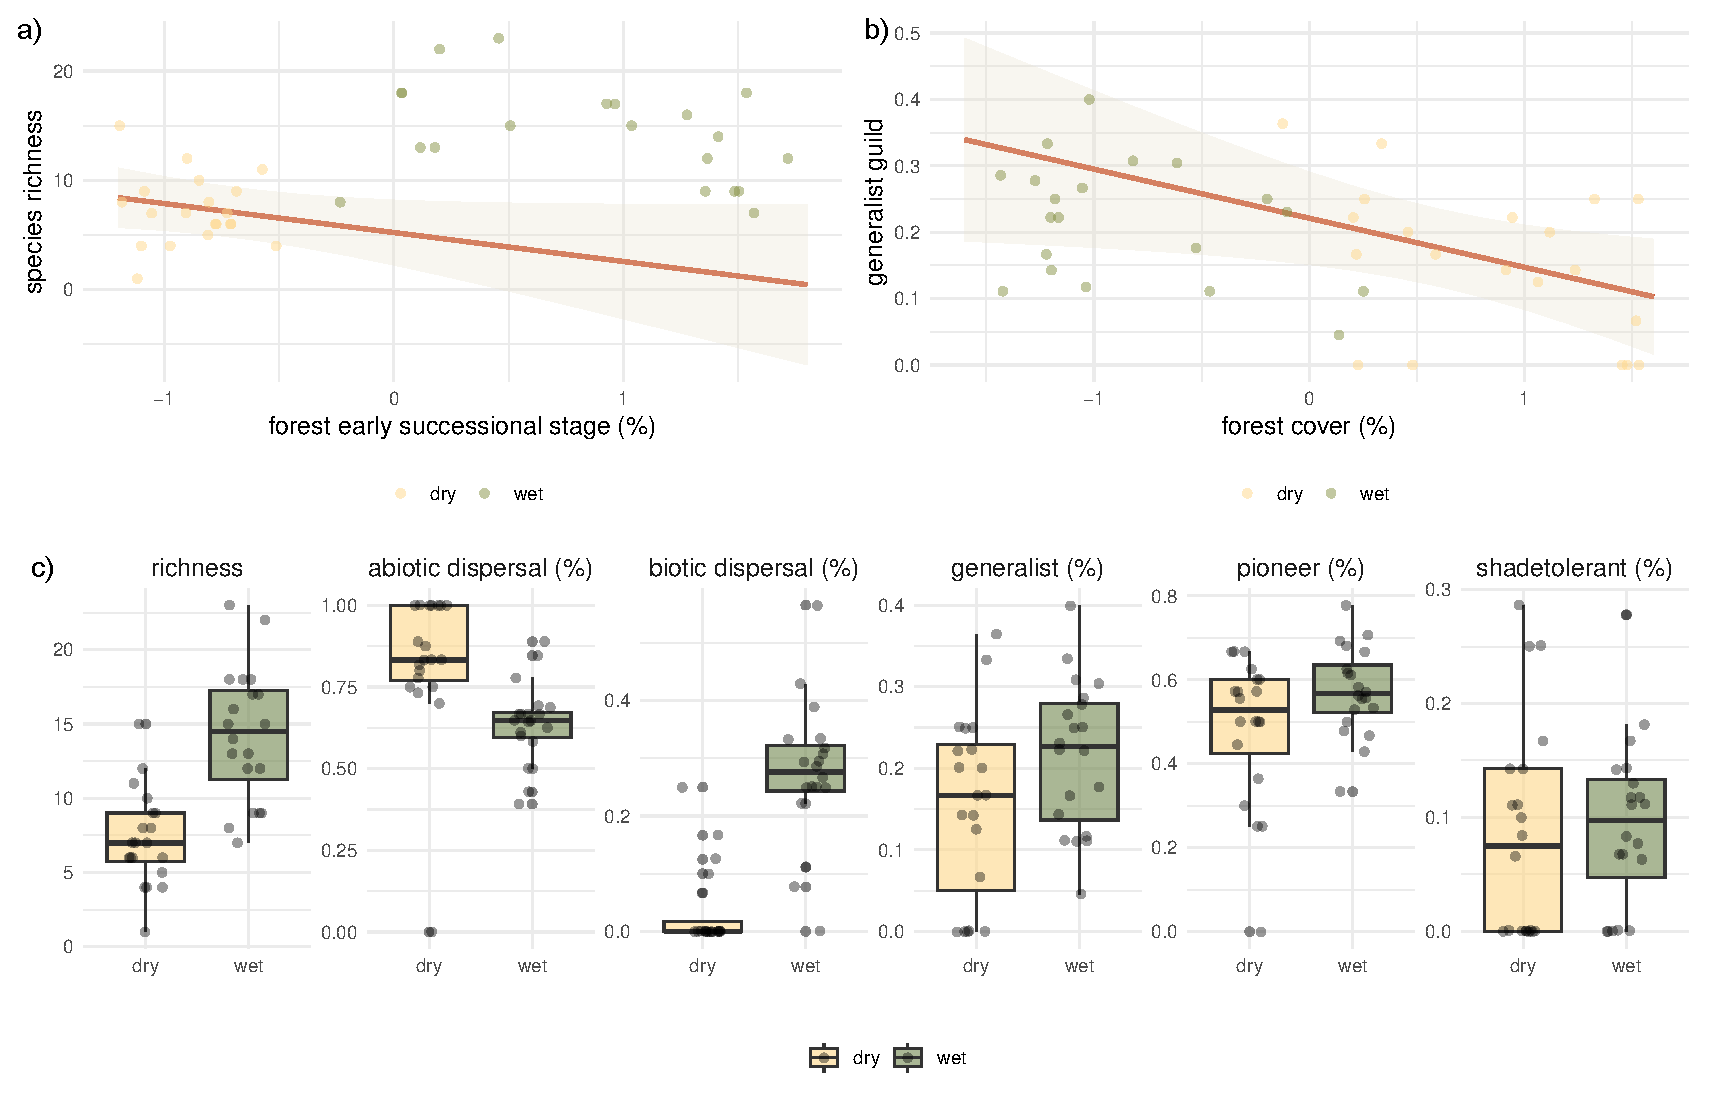
\includegraphics[width=\linewidth ,keepaspectratio]{Report/figures/11_stats.pdf}%
}
\caption{\textit{
%Graphical visualization of the models' statistically significant results. Figure a) illustrates the relationship between forest early successional stage and species richness ($\beta = -2.652, p < 0.1$). Figure b) illustrates the relationship between forest cover and generalist guild $(\beta = -0.074, p < 0.05)$. Figure a) and b) show scatterplots of raw data points with regression line representing model predictions. Figure c) illustrates the distribution of species richness ($\beta = 9.624$–$11.044$, $p < 0.01$), abiotic $(\beta = -0.473 - (-0.429), p < 0.01)$ and biotic $(\beta = 0.530 - 0.526, p < 0.01)$ dispersal, and generalist $(\beta = -0.071 - (-0.023), p > 0.1)$, pioneer $(\beta = 0.042 - 0.067, p > 0.1)$ and shade-tolerant $(\beta = 0.448 - 0.501, p > 0.1)$  guild in dry and wet tropical forest (N = 40).
Significant model results: (a) early successional stage  vs. species richness ($\beta = -2.652, p < 0.1$); (b) forest cover vs. generalist guild $(\beta = -0.074, p < 0.05)$. Scatterplots show raw data with regression lines as model predictions. 
(c) Distributions of species richness ($\beta = 9.624$–$11.044$, $p < 0.01$), abiotic $(\beta = -0.473 - (-0.429), p < 0.01)$ and biotic $(\beta = 0.526 - 0.530, p < 0.01)$ dispersal, and generalist $(\beta = -0.071 - (-0.023), p > 0.1)$, pioneer $(\beta = 0.042 - 0.067, p > 0.1)$ and shade-tolerant $(\beta = 0.448 - 0.501, p > 0.1)$  guild in dry and wet forests (N = 40).
}}
\label{fig:stats}
\end{figure}

